\documentclass{beamer}
\usepackage[utf8]{inputenc}

\usetheme{Madrid}
\usecolortheme{default}
\usepackage{amsmath,amssymb,amsfonts,amsthm}
\usepackage{txfonts}
\usepackage{tkz-euclide}
\usepackage{listings}
\usepackage{adjustbox}
\usepackage{array}
\usepackage{tabularx}
\usepackage{gvv}
\usepackage{lmodern}
\usepackage{circuitikz}
\usepackage{tikz}
\usepackage{graphicx}

\setbeamertemplate{page number in head/foot}[totalframenumber]

\usepackage{tcolorbox}
\tcbuselibrary{minted,breakable,xparse,skins}



\definecolor{bg}{gray}{0.95}
\DeclareTCBListing{mintedbox}{O{}m!O{}}{%
	breakable=true,
	listing engine=minted,
	listing only,
	minted language=#2,
	minted style=default,
	minted options={%
		linenos,
		gobble=0,
		breaklines=true,
		breakafter=,,
		fontsize=\small,
		numbersep=8pt,
		#1},
	boxsep=0pt,
	left skip=0pt,
	right skip=0pt,
	left=25pt,
	right=0pt,
	top=3pt,
	bottom=3pt,
	arc=5pt,
	leftrule=0pt,
	rightrule=0pt,
	bottomrule=2pt,
	toprule=2pt,
	colback=bg,
	colframe=orange!70,
	enhanced,
	overlay={%
		\begin{tcbclipinterior}
			\fill[orange!20!white] (frame.south west) rectangle ([xshift=20pt]frame.north west);
	\end{tcbclipinterior}},
	#3,
}
\lstset{
	language=C,
	basicstyle=\ttfamily\small,
	keywordstyle=\color{blue},
	stringstyle=\color{orange},
	commentstyle=\color{green!60!black},
	numbers=left,
	numberstyle=\tiny\color{gray},
	breaklines=true,
	showstringspaces=false,
}
%------------------------------------------------------------
%This block of code defines the information to appear in the
%Title page
\title %optional
{1.10.9}
%\subtitle{A short story}

\author % (optional)
{Hema Havil - EE25BTECH11050}



\begin{document}
	
	\frame{\titlepage}
	\begin{frame}{Question}
		Find the unit vector in the direction of the vector PQ, where P and Q are the points (1, 2, 3) and (4, 5, 6), respectively.
	\end{frame}

	
\begin{frame}{Theoretical Solution}
	Given,\\
         The points: 
         \begin{align}
             \vec{P}=\myvec{1\\2\\3} \vec{Q}=\myvec{4\\5\\6}
         \end{align}
         Let the required unit vector be $\vec{x}$, then\\ 
         The formula for unit vector along a line joining two points
         \begin{align}
             \vec{x}=\frac{\vec{X}}{\norm{\vec{X}}}
         \end{align}
         The vector along $\vec{P}$ and $\vec{Q}$ is\\
         \begin{align}
             \vec{X}=\vec{Q}-\vec{P}
         \end{align}
\end{frame}
\begin{frame}{Theoretical Solution}
\begin{align}
             \vec{X}=\myvec{4\\5\\6}-\myvec{1\\2\\3}
         \end{align}
         \begin{align}
             \vec{X}=\myvec{4-1\\5-2\\6-3}
         \end{align}
         \begin{align}
             \vec{X}=\myvec{3\\3\\3}
         \end{align}
         Magnitude of the vector $\vec{X}$ is\\
         \begin{align}
             \norm{\vec{X}}=\sqrt{X^T X}
         \end{align}
	\end{frame}
    \begin{frame}{Theoretical Solution}
        \begin{align}
             \norm{\vec{X}}=\sqrt{\myvec{3,3,3}\myvec{3\\3\\3}}
         \end{align}
         \begin{align}
             \norm{\vec{X}}=\sqrt{\brak{3}^2+\brak{3}^2+\brak{3}^2}
         \end{align}
         \begin{align}
             \norm{\vec{X}}=\sqrt{3\brak{3}^2}
         \end{align}
         \begin{align}
             \norm{\vec{X}}=3\sqrt{3}
         \end{align}
    \end{frame}
    \begin{frame}{Theoretical Solution}
        Then the unit vector,\\
         \begin{align}
             \vec{x}=\frac{1}{3\sqrt{3}}\brak{\vec{X}}=\frac{1}{3\sqrt{3}}\myvec{3\\3\\3}
         \end{align}
         \begin{align}
             \vec{x}=\frac{3}{3\sqrt{3}}\myvec{1\\1\\1}
         \end{align}
         \begin{align}
             \vec{x}=\myvec{\frac{1}{\sqrt{3}},\frac{1}{\sqrt{3}},\frac{1}{\sqrt{3}}}
         \end{align}
    \end{frame}
    \begin{frame}{Theoretical Solution}
        Therefore the required unit vector is\\
         \begin{align*}
             \vec{x}=\myvec{\frac{1}{\sqrt{3}},\frac{1}{\sqrt{3}},\frac{1}{\sqrt{3}}}
         \end{align*}
    \end{frame}
	
	\begin{frame}[fragile]
	\frametitle{C Code- Computing the unit vector}
	
	\begin{lstlisting}
// file: unitvec3d.c
#include <math.h>

#ifdef _WIN32
#define API __declspec(dllexport)
#else
#define API
#endif

// Compute unit vector from P to Q in 3D
// Inputs: P[3], Q[3]
// Output: unit[3]
// Returns: 0 on success, -1 if P=Q

	\end{lstlisting}
\end{frame}
\begin{frame}[fragile]
\frametitle{C Code - Computing the unit vector}
\begin{lstlisting}
    API int unit_vector_3d(const double* P, const double* Q, double* unit) {
    double dx = Q[0] - P[0];
    double dy = Q[1] - P[1];
    double dz = Q[2] - P[2];
    double norm = sqrt(dx*dx + dy*dy + dz*dz);
    if (norm == 0.0) return -1;
    unit[0] = dx / norm;
    unit[1] = dy / norm;
    unit[2] = dz / norm;
    return 0;
}
\end{lstlisting}
\end{frame}

\begin{frame}[fragile]
	\frametitle{Python Code using shared output}
	\begin{lstlisting}
		import ctypes, os, math
import matplotlib.pyplot as plt
from mpl_toolkits.mplot3d import Axes3D

# Load library
if os.name == "nt":
    libname = "unitvec3d.dll"
else:
    libname = "./libunitvec3d.so"
lib = ctypes.CDLL(libname)

# Function signature
lib.unit_vector_3d.argtypes = [
    ctypes.POINTER(ctypes.c_double),
    ctypes.POINTER(ctypes.c_double),
    ctypes.POINTER(ctypes.c_double),
]
	\end{lstlisting}
\end{frame}
\begin{frame}[fragile]
	\frametitle{Python Code using shared output}
	\begin{lstlisting}	
     lib.unit_vector_3d.restype = ctypes.c_int

def unit_vector_from_c(P, Q):
    P_arr = (ctypes.c_double * 3)(*P)
    Q_arr = (ctypes.c_double * 3)(*Q)
    U_arr = (ctypes.c_double * 3)()
    ret = lib.unit_vector_3d(P_arr, Q_arr, U_arr)
    if ret != 0:
        raise ValueError("P and Q coincide.")
    return [U_arr[0], U_arr[1], U_arr[2]]

# Example points
P = (1.0, 2.0, 3.0)
Q = (4.0, 5.0, 6.0)

	\end{lstlisting}
\end{frame}
\begin{frame}[fragile]
	\frametitle{Python Code using shared output}
	\begin{lstlisting}
# Get unit vector
u = unit_vector_from_c(P, Q)
PQ = [Q[i]-P[i] for i in range(3)]
print("Unit vector:", u)

# --- Plot ---
fig = plt.figure()
ax = fig.add_subplot(111, projection='3d')

# Plot points
ax.scatter(*P, color="red", s=60, label="P")
ax.scatter(*Q, color="blue", s=60, label="Q")

# Vector PQ
ax.quiver(P[0], P[1], P[2], PQ[0], PQ[1], PQ[2], color="green", label="PQ")

	\end{lstlisting}
\end{frame}
\begin{frame}[fragile]
        \frametitle{Python Code using shared output}
        \begin{lstlisting}
            # Unit vector (length 1)
ax.quiver(P[0], P[1], P[2], u[0], u[1], u[2], color="orange", label="Unit vector")

ax.set_xlabel('X')
ax.set_ylabel('Y')
ax.set_zlabel('Z')
ax.legend()
plt.show()
        \end{lstlisting}
\end{frame}
\begin{frame}{Plot by python using shared output from c}
	\begin{center}
	\begin{figure}[H]
		\centering
		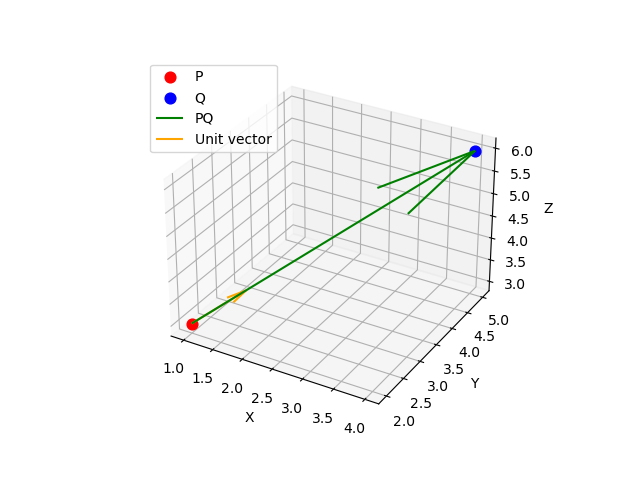
\includegraphics[width = 0.7\columnwidth]{figs/fig21.png}
		\caption{Plot of the unit vector along PQ}
		\label{fig1}
	\end{figure}
	\end{center}
\end{frame}
\begin{frame}[fragile]
     \frametitle{Python code for the plot}
\begin{lstlisting}
    import math
import matplotlib.pyplot as plt
from mpl_toolkits.mplot3d import Axes3D

def unit_vector(P, Q):
    """Compute unit vector from P to Q in 3D."""
    dx, dy, dz = Q[0]-P[0], Q[1]-P[1], Q[2]-P[2]
    norm = math.sqrt(dx*dx + dy*dy + dz*dz)
    if norm == 0:
        raise ValueError("P and Q are the same point, unit vector undefined.")
    return (dx/norm, dy/norm, dz/norm)

# Example points
P = (1, 2, 3)
Q = (4, 5, 6)
\end{lstlisting}
\end{frame}
\begin{frame}[fragile]
   \frametitle{Python code for the plot}
    \begin{lstlisting}
# Compute vector PQ and unit vector
PQ = (Q[0]-P[0], Q[1]-P[1], Q[2]-P[2])
u = unit_vector(P, Q)

print("Vector PQ =", PQ)
print("Unit vector =", u)

# --- Plot ---
fig = plt.figure()
ax = fig.add_subplot(111, projection='3d')

# Plot points
ax.scatter(*P, color="red", s=60, label="P")
ax.scatter(*Q, color="blue", s=60, label="Q")

# Vector PQ (green arrow)
ax.quiver(P[0], P[1], P[2], PQ[0], PQ[1], PQ[2],
          color="green", label="PQ", arrow_length_ratio=0.1)
 \end{lstlisting}
\end{frame}
 \begin{frame}[fragile]
       \frametitle{Python code for plot}
       \begin{lstlisting}
      # Unit vector (orange arrow, length 1)
ax.quiver(P[0], P[1], P[2], u[0], u[1], u[2],
          color="orange", label="Unit vector", arrow_length_ratio=0.2)

# Labels and aesthetics
ax.set_xlabel("X")
ax.set_ylabel("Y")
ax.set_zlabel("Z")
ax.legend()
ax.set_title("Vector PQ and Unit Vector from P")
ax.grid(True)

plt.show()
    \end{lstlisting}
 \end{frame}
 \begin{figure}
     \centering
     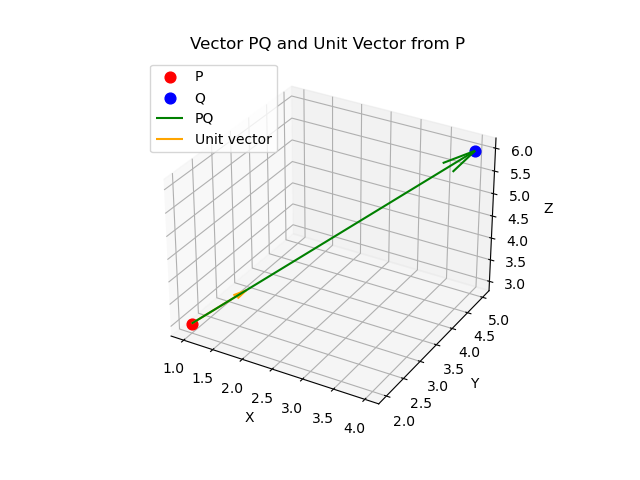
\includegraphics[width=0.7\linewidth]{figs/fig22.png}
     \caption{Plot for the unit vector along PQ}
     \label{fig2}
 \end{figure}
\end{document}
